% Generated by ops/build_paper_portfolio_withdrawals.py; do not edit numbers.
\section{Portfolio Survival under Withdrawn Options}
\label{app:portfolio-withdrawals}
A portfolio survives a withdrawn option if at least one of its solutions
remains valid. We evaluate survival across all five domains in 474 terminal checkpoint evaluations, each
with 128 prompts and four groups of eight responses per prompt. The groups have
overlapping sampling streams (App.~\ref{app:conditional-concentration}). Replay's
largest gains in expected distinct modes at four verified draws occur in
\texttt{Graph}, \texttt{Countdown}, \texttt{Python} and \texttt{PantryPlan}. Across 38 matched
domain--scale--level--objective comparisons,
\pmd{} gains correlate with survival gains at four verified draws
(Pearson $r=.57$).

\paragraph{Task perturbations.} Each task loses one option: a colour at one
vertex (\texttt{Graph}), an arithmetic operation (\texttt{Countdown}), a returned divisor value
(\texttt{Python}), a menu action (\texttt{MathIR}), or an ingredient (\texttt{PantryPlan}; see
App.~\ref{app:pantry-adaptation}). Options are enumerated from the task
specification. The solution-mode enumeration matches the certified counts for
all 1{,}280 prompts. A surviving certified mode establishes feasibility.
When the certified count is only a lower bound on the verifier's full support,
absence of a surviving mode from the enumeration does not establish infeasibility. Of
9{,}864 options, 9{,}118 retain at least one certified mode. Among these,
8{,}308 are binding: they also remove at least one certified mode. We evaluate
both the binding set and the full set with a feasibility certificate.

\paragraph{Survival criterion.} Each portfolio contains the verified
responses among eight draws. It survives when at least one of these solutions
remains valid after the option is removed. \texttt{Graph}, \texttt{Countdown} and \texttt{Python} determine this directly from
the outcome key, including verified keys outside the enumeration. \texttt{Countdown}
contributes 2 such keys, observed 50 times among the
846{,}398 verified draws in this evaluation: the verifier accepts unary negation, which the
expression enumeration omits. For \texttt{MathIR}, re-enumerating the reduced menu tests
whether the same executed state path remains realizable, possibly through a
different action sequence. For \texttt{PantryPlan}, we test the certified plan
associated with each ingredient-support key. All observed \texttt{MathIR} and \texttt{PantryPlan} keys belong to their
respective enumerations.

\paragraph{Survival conditional on correct draws.} Raw survival depends on
both correctness and the distribution of valid modes. At budgets $m=1,2,4$, we
compute the exact expected survival of a uniformly selected $m$-element subset
of a portfolio's verified draws, as in App.~\ref{app:cross-model-overlap}.
Replay--control contrasts use only prompt--group pairs with at least $m$
verified draws under both methods, so eligibility can change with $m$.
Fixing the number of correct draws does not equalize policy accuracy.
A survival difference can also arise because the modes one method favors are
individually more robust to withdrawals, so a gain that grows with $m$ does
not by itself isolate the contribution of diversity. Expected distinct modes
at the same budget therefore serve as a separate measure of portfolio breadth.

\begin{table}[!htbp]
\centering
\caption{\textbf{Binding withdrawals remove certified modes while retaining a feasibility certificate.} Each row covers 128 prompts. Support is the mean certified mode count per prompt; Options counts single withdrawals. Binding counts options that retain at least one certified mode and remove at least one. Kept is the mean retained fraction of certified modes across binding options. Pairs counts binding pairs of withdrawals, and Kept$_2$ gives the corresponding retained fraction.}
\label{tab:withdrawal-inventory}
\scriptsize
\setlength{\tabcolsep}{3pt}
\begin{tabular}{llrrrrrrr}
\toprule
Domain & Level & Prompts & Support & Options & Binding & Kept & Pairs & Kept$_2$ \\
\midrule
\texttt{Graph} & 1 & 128 & 6.3 & 1152 & 818 & 0.57 & 1957 & 0.34 \\
\texttt{Graph} & 2 & 128 & 6.1 & 1536 & 1068 & 0.57 & 3457 & 0.35 \\
\texttt{Countdown} & 1 & 128 & 4.5 & 512 & 147 & 0.48 & 21 & 0.44 \\
\texttt{Countdown} & 2 & 128 & 4.4 & 512 & 185 & 0.49 & 40 & 0.37 \\
\texttt{Python} & 1 & 128 & 229.4 & 1433 & 1433 & 0.68 & 7716 & 0.50 \\
\texttt{Python} & 2 & 128 & 251.7 & 1647 & 1647 & 0.71 & 10381 & 0.55 \\
\texttt{MathIR} & 1 & 128 & 5.0 & 768 & 448 & 0.40 & 384 & 0.23 \\
\texttt{MathIR} & 2 & 128 & 5.0 & 768 & 512 & 0.45 & 512 & 0.25 \\
\texttt{PantryPlan} & 1 & 128 & 18.2 & 768 & 651 & 0.44 & 1231 & 0.18 \\
\texttt{PantryPlan} & 2 & 128 & 18.2 & 768 & 653 & 0.45 & 1228 & 0.19 \\
\bottomrule
\end{tabular}
\end{table}
\begin{table}[!htbp]
\centering
\caption{\textbf{Both replay arms improve four-draw survival in \texttt{Graph}, \texttt{Python} and \texttt{PantryPlan}.} Each replay arm is compared with its fresh-objective control. Survival differences are percentage points; $\Delta D_4$ is the difference in expected distinct modes at four verified draws. Raw uses all eight responses; Budget columns use the indicated number of verified draws. Fixed-correct-draw results pool jointly eligible prompt--group pairs across matched seeds, scales and levels; raw results use all paired groups. All columns use binding options except Budget 4 (all), which includes every option with a feasibility certificate. Brackets are pointwise 95\% intervals from 20{,}000 paired bootstrap replicates. Each resampled cluster is a prompt within one level and scale, with its groups and seeds kept together; copies at other scales are separate clusters. Intervals condition on the observed seeds.}
\label{tab:withdrawal-contrasts}
\scriptsize
\setlength{\tabcolsep}{3pt}
\begin{tabular}{llrrrrrr}
\toprule
Domain & Arm & Raw & Budget 1 & Budget 2 & Budget 4 & Budget 4 (all) & $\Delta D_4$ \\
\midrule
\texttt{Graph} & Re:Dr & $34.78$ & $0.00$ $[0.00, 0.00]$ & $10.51$ $[8.76, 12.31]$ & $19.65$ $[15.61, 23.82]$ & $15.66$ & 1.290 \\
\texttt{Graph} & Re:Max & $18.98$ & $0.00$ $[0.00, 0.00]$ & $6.62$ $[5.23, 7.98]$ & $10.99$ $[8.25, 13.81]$ & $8.31$ & 0.646 \\
\texttt{Countdown} & Re:Dr & $5.32$ & $3.51$ $[1.88, 5.30]$ & $6.52$ $[4.27, 8.94]$ & $9.58$ $[6.81, 12.63]$ & $2.53$ & 0.626 \\
\texttt{Countdown} & Re:Max & $1.95$ & $-2.40$ $[-4.62, -0.21]$ & $-1.25$ $[-3.70, 1.14]$ & $0.10$ $[-2.62, 2.78]$ & $-0.05$ & 0.490 \\
\texttt{Python} & Re:Dr & $38.99$ & $-0.22$ $[-1.25, 0.91]$ & $4.09$ $[3.17, 5.08]$ & $7.67$ $[6.82, 8.58]$ & $7.67$ & 0.317 \\
\texttt{Python} & Re:Max & $22.84$ & $1.53$ $[0.87, 2.24]$ & $3.85$ $[3.04, 4.72]$ & $5.68$ $[4.80, 6.64]$ & $5.68$ & 0.198 \\
\texttt{MathIR} & Re:Dr & $33.61$ & $0.01$ $[0.00, 0.05]$ & $0.12$ $[0.03, 0.23]$ & $0.14$ $[0.00, 0.30]$ & $0.08$ & 0.004 \\
\texttt{MathIR} & Re:Max & $21.64$ & $0.00$ $[-0.04, 0.05]$ & $0.03$ $[-0.03, 0.10]$ & $0.09$ $[-0.01, 0.21]$ & $0.06$ & 0.003 \\
\texttt{PantryPlan} & Re:Dr & $16.55$ & $-1.11$ $[-1.65, -0.54]$ & $4.36$ $[3.82, 4.87]$ & $9.78$ $[8.90, 10.65]$ & $9.20$ & 0.810 \\
\texttt{PantryPlan} & Re:Max & $13.04$ & $-0.64$ $[-1.04, -0.21]$ & $3.12$ $[2.72, 3.53]$ & $6.61$ $[5.83, 7.39]$ & $6.20$ & 0.547 \\
\bottomrule
\end{tabular}
\end{table}
Raw survival improves in 39 of 40 domain--scale--level--objective
comparisons. At four verified draws, the point estimate is positive in
28 of 39 eligible comparisons; these conditional comparisons cover
fewer prompt--group pairs than raw survival. Outside \texttt{MathIR}, Re:Dr adds between
$.3$ and $1.3$ expected distinct modes at four verified draws, and its pooled
survival gains reach 19.6 percentage points. In \texttt{MathIR}, the corresponding
gains are only $.004$ distinct modes and $.14$ survival points, with an interval
of $[.00,.30]$ after rounding. These small positive estimates are consistent
with the small \pmd{} gain in Table~\ref{tab:cross-scale-terminal-effects}.

\texttt{Graph}'s one-draw contrast is zero by construction. Each binding withdrawal
removes one color at one vertex, and each valid coloring is excluded by
exactly one such withdrawal per variable vertex, so every individual mode
survives the same fraction of binding withdrawals. Including nonbinding options shrinks the contrasts,
because those options leave every certified mode intact; for example,
63\% of \texttt{Countdown} Level-1 options with a feasibility certificate are nonbinding.
The Budget 4 (all) and binding columns therefore describe different withdrawal
populations.
\begin{figure}[!htbp]
  \centering
  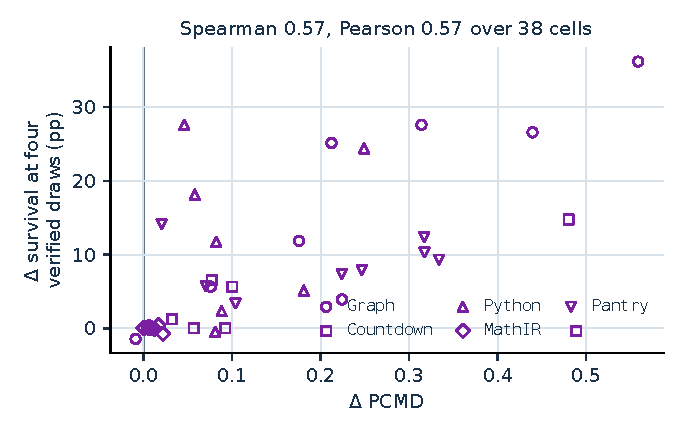
\includegraphics[width=0.62\linewidth]{figures/withdrawal_pmd_agreement.pdf}
  \caption{\textbf{Diversity gains correlate with survival gains after a withdrawal.} Each mark is one replay--fresh-objective contrast in a domain, scale and level. The horizontal axis is the terminal \pmd{} difference; the vertical axis is the percentage-point survival difference at four verified draws, averaged equally over eligible seed-specific contrasts. Survival uses jointly eligible prompt--group pairs within each seed. Marker shape identifies the domain; zero lines mark no change. The 38 comparisons have Pearson and Spearman correlations of $.57$; points show estimates without intervals. The association is descriptive, and the two metrics need not use the same eligible population.}
  \label{fig:withdrawal-pmd-agreement}
\end{figure}

\subsection{Two withdrawals at once}
\label{app:withdrawal-severity}
We next remove two binding options at once. Of the 29{,}213 pairs of binding
single withdrawals, 26{,}927 retain at least one certified mode and enter the
survival comparison. For \texttt{Graph}, \texttt{Countdown}, \texttt{Python} and \texttt{PantryPlan},
a certified mode survives the pair exactly when it survives both individual
withdrawals. \texttt{MathIR} can differ: removing two actions can eliminate every
realization of a state path even when either action alone can be removed.
Re-enumerating the reduced menus shows that no such case occurs here: for all
1{,}344 \texttt{MathIR} pairs, including those that leave no certified mode,
the surviving set equals the intersection of the two single-withdrawal sets.

\begin{table}[!htbp]
\centering
\caption{\textbf{Two withdrawals retain survival gains in \texttt{Graph}, \texttt{Python} and \texttt{PantryPlan}.} Entries are replay--fresh-objective differences in percentage points at two (@2) or four (@4) verified draws. One uses binding single options; Two uses binding pairs with a feasibility certificate. Their eligible prompt populations can differ. Estimates pool jointly eligible groups. Brackets are pointwise 95\% paired prompt-bootstrap intervals with the clustering in Table~\ref{tab:withdrawal-contrasts}.}
\label{tab:withdrawal-severity}
\scriptsize
\setlength{\tabcolsep}{3pt}
\begin{tabular}{llrrrr}
\toprule
Domain & Arm & One @2 & One @4 & Two @2 & Two @4 \\
\midrule
\texttt{Graph} & Re:Dr & $10.51$ & $19.65$ $[15.61, 23.82]$ & $10.02$ & $23.65$ $[19.14, 28.25]$ \\
\texttt{Graph} & Re:Max & $6.62$ & $10.99$ $[8.25, 13.81]$ & $5.93$ & $12.51$ $[9.37, 15.69]$ \\
\texttt{Countdown} & Re:Dr & $6.52$ & $9.58$ $[6.81, 12.63]$ & $3.29$ & $6.11$ $[0.87, 12.22]$ \\
\texttt{Countdown} & Re:Max & $-1.25$ & $0.10$ $[-2.62, 2.78]$ & $-5.53$ & $-4.87$ $[-11.80, 0.76]$ \\
\texttt{Python} & Re:Dr & $4.09$ & $7.67$ $[6.82, 8.58]$ & $5.37$ & $10.10$ $[8.77, 11.55]$ \\
\texttt{Python} & Re:Max & $3.85$ & $5.68$ $[4.80, 6.64]$ & $5.64$ & $8.16$ $[6.79, 9.64]$ \\
\texttt{MathIR} & Re:Dr & $0.12$ & $0.14$ $[0.00, 0.30]$ & $0.18$ & $0.20$ $[0.01, 0.45]$ \\
\texttt{MathIR} & Re:Max & $0.03$ & $0.09$ $[-0.01, 0.21]$ & $0.04$ & $0.12$ $[-0.01, 0.29]$ \\
\texttt{PantryPlan} & Re:Dr & $4.36$ & $9.78$ $[8.90, 10.65]$ & $2.85$ & $7.23$ $[6.51, 7.95]$ \\
\texttt{PantryPlan} & Re:Max & $3.12$ & $6.61$ $[5.83, 7.39]$ & $2.03$ & $4.94$ $[4.35, 5.57]$ \\
\bottomrule
\end{tabular}
\end{table}

Two withdrawals retain less certified support on average
(Table~\ref{tab:withdrawal-inventory}). Re:Dr's pooled survival gain at four
verified draws rises in \texttt{Graph}, \texttt{Python} and \texttt{MathIR}, and falls in \texttt{Countdown} and
\texttt{PantryPlan}. \texttt{Countdown} Level 1 starts with only 4.5 certified modes per prompt;
\texttt{PantryPlan} Level 1 retains only 18\% of its certified modes under a binding pair.
These support differences coincide with the smaller gains but do not
establish their cause. Across domain--scale--level--objective comparisons,
25 of 39 point estimates are positive at four verified draws,
compared with 28 of 39 for single withdrawals.

\subsection{Decoding settings as a substitute}
\label{app:withdrawal-decoding}
Can a better decoding setting give an ordinary policy the same survival?
We evaluate binding Level-1 withdrawals on 128 prompts per domain, using the
separate Qwen2.5-0.5B cohort trained for twelve passes in
App.~\ref{app:decoding-objection}. Its replay variant combines separate mass
and within-buffer balancing terms with novelty and semantic-entropy shaping;
it differs from Re:Dr in both objective and training duration. Five seeds per
arm are evaluated at 11 settings: six temperatures from $.5$ to $2.0$,
three settings with larger groups, and two with top-$p=.95$. Larger groups
increase $K$ from 8 to 32, but use two groups rather than four: total responses
per prompt double from 32 to 64. The reference is $T=1$, top-$p=1$, and four
groups of eight. For each domain, we select the control setting with the
highest four-verified-draw survival on these evaluation prompts, while replay
keeps the reference setting.

\begin{table}[!htbp]
\centering
\caption{\textbf{Replay survival exceeds the selected control setting in all five domains.} Survival at four verified draws is expressed as percentages. Control, Control grid and Replay are equal-seed means on each setting's own eligible groups; the grid column gives the control range and Best its maximizing temperature. $\Delta$ instead pools jointly eligible groups for reference replay minus selected control, so it need not equal the difference of the displayed means. Brackets are pointwise 95\% intervals from 20{,}000 paired prompt-bootstrap replicates, keeping all groups and five seeds of a prompt together. The selected setting stays fixed in the bootstrap; intervals condition on that selection and the seeds.}
\label{tab:withdrawal-decoding}
\scriptsize
\setlength{\tabcolsep}{3pt}
\begin{tabular}{lrrcrr}
\toprule
Domain & Control & Control grid & Best & Replay & $\Delta$ vs best \\
\midrule
\texttt{Graph} & 58.61 & 58.59--58.85 & $T{=}2$ & 95.91 & $36.97$ $[35.53, 38.42]$ \\
\texttt{Countdown} & 15.49 & 12.57--16.16 & $T{=}1.6$ & 40.09 & $28.87$ $[18.98, 38.87]$ \\
\texttt{Python} & 70.54 & 70.36--70.54 & $T{=}0.5$ & 77.56 & $8.33$ $[7.15, 9.69]$ \\
\texttt{MathIR} & 72.23 & 72.18--72.55 & $T{=}2$ & 73.60 & $1.37$ $[0.61, 2.30]$ \\
\texttt{PantryPlan} & 50.65 & 50.02--51.79 & $T{=}2$ & 64.09 & $12.73$ $[10.22, 15.31]$ \\
\bottomrule
\end{tabular}
\end{table}

Control survival spans at most 3.6 percentage points across the grid.
The paired replay gains range from 1.4 to 37.0 points, with all five
pointwise intervals above zero. Every selected control setting changes only the
temperature, keeping eight-response groups and top-$p=1$. The tested decoding
changes therefore do not close the survival gap in this cohort. Because each
control setting is selected on the evaluation prompts, the control's survival
is, if anything, optimistic for new prompts. Finite samples cannot show that
the missing alternative modes have zero probability under the control.

\subsection{Recovery after a withdrawal}
\label{app:withdrawal-recovery}
Recovery is evaluated at the Level-1 Qwen2.5-0.5B terminal Dr.GRPO and Re:Dr
checkpoints from two matched training seeds in each of five domains. Each domain has 32 test and 16 temperature-calibration prompts in a
disjoint split. Prompts without a binding withdrawal that retains a certified
mode are excluded, leaving 28 test and 15 calibration prompts in \texttt{Countdown} and all
prompts elsewhere. Up to four binding options per test prompt give
533 distinct withdrawals, shared by both arms and seeds.

Each initial portfolio contains eight responses. Ordinary sampling uses its
terminal evaluation group at $T=1$. The temperature strategy generates a group
at the temperature in $\{.7,1.0,1.3\}$ maximizing mean survival on the
calibration prompts. The diversity-prompt strategy generates the eight
responses sequentially, with the preceding responses included in each request.
All strategies share the same recovery procedure. If no initial mode survives,
the model generates one response per call at $T=1$, for up to eight calls,
with the revised task, the initial portfolio and previous failed attempts in
context. Recovery stops at the first verified response whose mode survives the
withdrawal.

Survival uses the mode predicates defined above. In \texttt{MathIR}, a retained or newly
generated state path can count as surviving even if realizing it under the
reduced menu requires a different action sequence. \texttt{PantryPlan} responses are
six-bit ingredient-support masks projected onto verified quantities by the
environment (App.~\ref{app:prompt-pantry}); survival is evaluated on the resulting
support key. These outcomes therefore measure whether a mode remains feasible,
not whether the original response text can be reused unchanged.

\begin{table}[!htbp]
\centering
\caption{\textbf{Replay improves ordinary and temperature-tuned recovery in every domain.} Saved is the percentage of withdrawals with a surviving initial mode; By 8 also counts those resolved within eight additional responses. Calls is the mean additional response count, with zero for initial survival and eight for unresolved cases. Each row pools the same withdrawals over two matched seeds. Fresh is Dr.GRPO and Replay is Re:Dr; the three strategies differ only in initial portfolio generation.}
\label{tab:withdrawal-recovery}
\scriptsize
\setlength{\tabcolsep}{3pt}
\begin{tabular}{llrrrrrr}
\toprule
Domain & Strategy & Fresh saved & Fresh by 8 & Fresh calls & Replay saved & Replay by 8 & Replay calls \\
\midrule
\texttt{Graph} & Ordinary & 15.62 & 22.66 & 6.38 & 83.20 & 91.02 & 1.01 \\
\texttt{Graph} & Tuned temperature & 15.62 & 20.31 & 6.55 & 77.34 & 89.06 & 1.36 \\
\texttt{Graph} & Diversity prompt & 29.69 & 30.47 & 5.58 & 62.50 & 74.61 & 2.44 \\
\texttt{Countdown} & Ordinary & 2.70 & 2.70 & 7.78 & 9.46 & 10.81 & 7.23 \\
\texttt{Countdown} & Tuned temperature & 2.70 & 2.70 & 7.78 & 9.46 & 13.51 & 7.05 \\
\texttt{Countdown} & Diversity prompt & 2.70 & 2.70 & 7.78 & 5.41 & 9.46 & 7.41 \\
\texttt{Python} & Ordinary & 14.06 & 14.06 & 6.88 & 69.92 & 77.73 & 2.21 \\
\texttt{Python} & Tuned temperature & 14.06 & 14.06 & 6.88 & 71.88 & 75.78 & 2.12 \\
\texttt{Python} & Diversity prompt & 14.06 & 14.06 & 6.88 & 62.50 & 67.97 & 2.79 \\
\texttt{MathIR} & Ordinary & 38.39 & 44.20 & 4.60 & 58.93 & 65.18 & 2.92 \\
\texttt{MathIR} & Tuned temperature & 37.05 & 45.09 & 4.61 & 63.84 & 67.86 & 2.67 \\
\texttt{MathIR} & Diversity prompt & 41.07 & 45.09 & 4.58 & 47.32 & 53.57 & 3.85 \\
\texttt{PantryPlan} & Ordinary & 31.25 & 31.64 & 5.48 & 47.66 & 52.34 & 4.04 \\
\texttt{PantryPlan} & Tuned temperature & 31.25 & 44.53 & 4.81 & 53.12 & 62.11 & 3.38 \\
\texttt{PantryPlan} & Diversity prompt & 56.64 & 58.20 & 3.39 & 33.98 & 45.70 & 4.71 \\
\bottomrule
\end{tabular}
\end{table}


\begin{table}[!htbp]
\centering
\caption{\textbf{Recovery benefits depend on the initial portfolio strategy.} Entries are paired Re:Dr--Dr.GRPO differences on the same withdrawals under each strategy. Saved and By 8 are percentage points; Calls is additional responses. Brackets are pointwise 95\% intervals from 20{,}000 paired prompt-bootstrap replicates. Each prompt's withdrawals and both training seeds move together; intervals condition on those two matched training seeds.}
\label{tab:withdrawal-recovery-contrast}
\scriptsize
\setlength{\tabcolsep}{3pt}
\begin{tabular}{llrrr}
\toprule
Domain & Strategy & $\Delta$ saved & $\Delta$ by 8 & $\Delta$ calls \\
\midrule
\texttt{Graph} & Ordinary & $67.58$ $[57.81, 76.56]$ & $68.36$ $[59.38, 76.95]$ & $-5.37$ $[-6.05, -4.65]$ \\
\texttt{Graph} & Tuned temperature & $61.72$ $[51.95, 71.09]$ & $68.75$ $[61.33, 75.78]$ & $-5.20$ $[-5.84, -4.52]$ \\
\texttt{Graph} & Diversity prompt & $32.81$ $[21.09, 44.14]$ & $44.14$ $[34.77, 53.12]$ & $-3.14$ $[-3.95, -2.30]$ \\
\texttt{Countdown} & Ordinary & $6.76$ $[1.35, 13.89]$ & $8.11$ $[1.43, 16.18]$ & $-0.55$ $[-1.12, -0.11]$ \\
\texttt{Countdown} & Tuned temperature & $6.76$ $[1.35, 13.89]$ & $10.81$ $[3.33, 19.32]$ & $-0.73$ $[-1.35, -0.21]$ \\
\texttt{Countdown} & Diversity prompt & $2.70$ $[0.00, 6.58]$ & $6.76$ $[1.32, 13.64]$ & $-0.38$ $[-0.76, -0.06]$ \\
\texttt{Python} & Ordinary & $55.86$ $[44.92, 65.23]$ & $63.67$ $[51.56, 74.22]$ & $-4.67$ $[-5.45, -3.76]$ \\
\texttt{Python} & Tuned temperature & $57.81$ $[46.88, 67.19]$ & $61.72$ $[50.39, 71.48]$ & $-4.76$ $[-5.54, -3.87]$ \\
\texttt{Python} & Diversity prompt & $48.44$ $[37.11, 59.38]$ & $53.91$ $[41.80, 65.62]$ & $-4.09$ $[-4.99, -3.14]$ \\
\texttt{MathIR} & Ordinary & $20.54$ $[11.16, 30.09]$ & $20.98$ $[12.71, 29.82]$ & $-1.68$ $[-2.37, -1.02]$ \\
\texttt{MathIR} & Tuned temperature & $26.79$ $[18.26, 35.65]$ & $22.77$ $[13.89, 32.27]$ & $-1.94$ $[-2.66, -1.28]$ \\
\texttt{MathIR} & Diversity prompt & $6.25$ $[-4.09, 16.67]$ & $8.48$ $[-0.46, 18.26]$ & $-0.73$ $[-1.50, 0.03]$ \\
\texttt{PantryPlan} & Ordinary & $16.41$ $[8.20, 25.39]$ & $20.70$ $[11.72, 30.47]$ & $-1.44$ $[-2.18, -0.76]$ \\
\texttt{PantryPlan} & Tuned temperature & $21.88$ $[13.28, 31.25]$ & $17.58$ $[10.94, 24.61]$ & $-1.43$ $[-2.00, -0.91]$ \\
\texttt{PantryPlan} & Diversity prompt & $-22.66$ $[-31.25, -13.67]$ & $-12.50$ $[-21.88, -2.73]$ & $1.32$ $[0.55, 2.05]$ \\
\bottomrule
\end{tabular}
\end{table}

With ordinary or temperature-tuned initial portfolios, replay resolves more
withdrawals and uses fewer recovery responses in every domain. All ten
resolution contrasts and all ten response-count contrasts have pointwise
intervals excluding zero. With ordinary initial portfolios, replay needs
0.55 to 5.37 fewer recovery responses per withdrawal. Summed over all
three strategies and both seeds, replay uses 9{,}872 recovery responses and
the control uses 18{,}335. These totals cover recovery only, excluding initial
portfolios and temperature calibration, and response counts do not account for
token or context lengths or for training compute.

The diversity prompt increases the control's initial survival in \texttt{Graph} and
\texttt{PantryPlan} relative to ordinary sampling, with intervals above zero. For
replay, it lowers the initial-survival point estimate in every domain. The
intervention changes both the request for alternatives and the accumulated
context, and this design does not separate their effects. With both arms using
the diversity prompt, \texttt{PantryPlan} favors the control by 22.66 points of initial survival and 12.50 points of
resolution by eight calls. Replay's initial-survival difference is positive
in the other four domains, ranging from 2.7 to 48.4 points, although the
\texttt{Countdown} and \texttt{MathIR} intervals include zero. \texttt{PantryPlan}'s six-bit response format
permits enumerating support masks, but this comparison does not establish that
enumerability explains the reversal.

\paragraph{Interpretation and limits.} In \texttt{Graph}, \texttt{Countdown}, \texttt{Python} and \texttt{PantryPlan},
Re:Dr's broader four-draw portfolios accompany larger survival gains than in
\texttt{MathIR}. The positive association with \pmd{} is descriptive. Fixing the number
of verified draws conditions on jointly eligible groups; it does not fix policy
accuracy, and eligibility can change with the draw budget. An option enters
the analysis only when a certified mode survives it; where the certified count
is a lower bound on the verifier's support, some excluded options may also be
feasible. The interventions cover single and paired withdrawals rather than
arbitrary task revisions. Recovery outcomes rest on domain-specific mode
predicates, and \texttt{PantryPlan}'s ordering reverses under the diversity prompt. Finally, the intervals quantify prompt-sampling uncertainty within
the observed training cohorts; they do not estimate variability over new
training seeds.
